\def \ti{\textit}
\def \bf{\textbf}

\chapter{Generazione numeri pseudo-casuali}
	\label{cap:generatorerandom}

Per la generazione di numeri pseudo casuali, il simulatore implementato, utilizza il \textbf{Generatore di Lehmer} con le relative funzioni implementate all'interno delle librerie \textit{rngs} e \textit{rvms}. Nella fase di impostazione del simulatore (ovvero durante il lancio), viene chiesto all'utente di scegliere quale seed adoperare, in modo che il generatore possa elaborare numeri pseudo-casuali partendo da quest'ultimo.

\section{Generatore di Lehmer}
Il generatore di Lehmer è un generatore basato su un algoritmo che da origine ad una sequenza di numeri pseudo-casuali. \'E definito da due parametri:

\begin{itemize}
 \item un modulo m, che è un numero primo molto grande (in questo caso si è usato $2^{31} - 1$);
 \item un moltiplicatore a che rappresenta un numero intero compreso tra 1 ed m-1.
\end{itemize}

La sequenza numerica pseudo-random viene generata tramite la formula :

\begin{center} $x_{i+1} = ax_{i} mod m$ \end{center}

\noindent Questa sequenza parte da un numero $x_{0}$ detto seed, anch'esso scelto tra 1 ed m - 1. Non tutte le combinazioni di a ed m però sono ottimali per realizzare una sequenza di numeri che garantiscano una buona randomicità. Per vedere dunque se un seed e un moltiplicatore garantiscano un buon livello di randomicità esistono dei test empirici.

\section{Test degli estremi}
Il test scelto per verificare la correttezza dei numeri generati è quello conosciuto come ``\textit{Test degli estremi}''. Questo test si basa sul teorema seguente:

\vspace{0.5cm} \noindent \textbf{Teorema} Se $U_{0}^{}$, $U_{1}^{}$,...,$U_{d-1}^{}$ è una sequenza di variabili \textit{Uniform(0,1)} e se 

\begin{center}R = max{$U_{0}^{}$, $U_{1}^{}$,...,$U_{d-1}^{}$} \end{center} 

\noindent allora la variabile U = $R_{}^{d}$ è una \textit{Uniform(0,1)} \footnote{Attenzione: il teorema afferma che la variabile U è una Uniform(0,1), mentre la variabile R non lo è.}.

In pratica verifica che la variabilità delle altezze dell'istogramma prodotto dai numeri pseudo-casuali generati è sufficientemente piccola da poter concludere che questi numeri appartengano ad una popolazione \textit{Uniform(0,1)}. Questa operazione è fondamentale in quanto tutte le altre distribuzioni di probabilità contenute all'interno della libreria utilizzata vengono generati a partire dalla \textit{Uniform(0,1)}.

\section{Algoritmo}
Il comportamento del generatore può essere testato raggruppando gli output del generatore \textit{d} termini alla volta, trovando il massimo di ogni batch, elevando il massimo alla \textit{d}-esima potenza, e contando tutti i massimi così generati. Vediamo un esempio di questo algoritmo sotto forma di codice:

\begin{verbatim}
  for(stream = 0; stream < 256L; stream++) {
      long o[K];
      memset(o, 0, K * sizeof(long));
      for(i = 0; i < N; i++) {
          double r = Random();
          for(j = 1; j < D; j++) {
              u = Random();
              if(u > r) r = u;
          }
          u = exp(D * log(r));
          x = u * K;
          o[x] ++;
      }
  }
\end{verbatim}

Per effettuare correttamente questo test è necessario prendere $K >= 1000$, $N >= 10K$, $d >= 2$. Nel nostro caso abbiamo scelto $K = 5000$, $N = 100000$ e $d = 7$. Una volta selezionati i valori si procede all'esecuzione in questo modo:
\begin{itemize}
 \item Usare l'algoritmo precedentemente descritto per calcolare l'istogramma.
 \item Calcolare la statistica \textit{v} Chi-Quadro.
 \item Scegliere l'intervallo di confidenza che vogliamo verificare, nel nostro caso è al 95\%.
 \item Determinare le soglie critiche $v_{1}^{*}$ e $v_{2}^{*}$.
\end{itemize}
Se \textit{v $<$ $v_{1}^{*}$} o \textit{v $>$ $v_{2}^{*}$} il test è da considerarsi \textit{fallito}.

\section{Test e conclusioni}
\noindent Vediamo per prima cosa come si comporta il simulatore nel caso il seed sia 48271.

\begin{figure}[H]
  \centering
  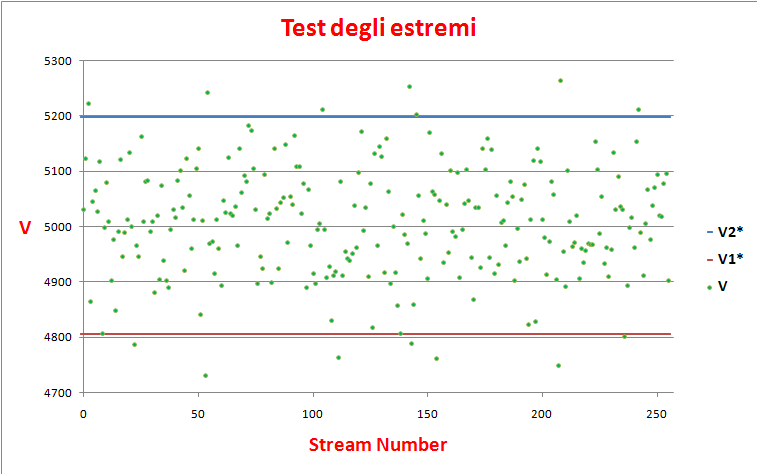
\includegraphics[scale=0.55]{img/result_48271.png}
  \caption[Test degli estremi]{SEED 48271.}
  \label{fig:result_48271}
\end{figure}

\noindent Oltre al seed proposto il test è stato eseguito anche sui seguenti:
\begin{itemize}
\item 615425336
\begin{figure}[H]
  \centering
  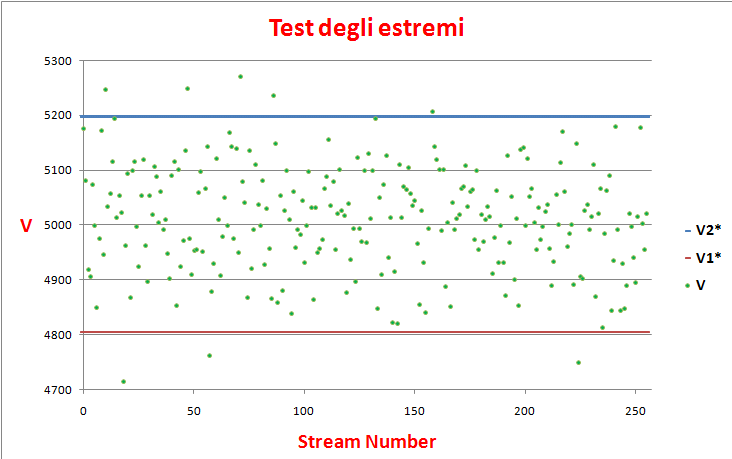
\includegraphics[scale=0.55]{img/result_615425336.png}
  \caption[Test degli estremi]{SEED 615425336.}
  \label{fig:result_615425336}
\end{figure}
\item 37524306
\begin{figure}[H]
  \centering
  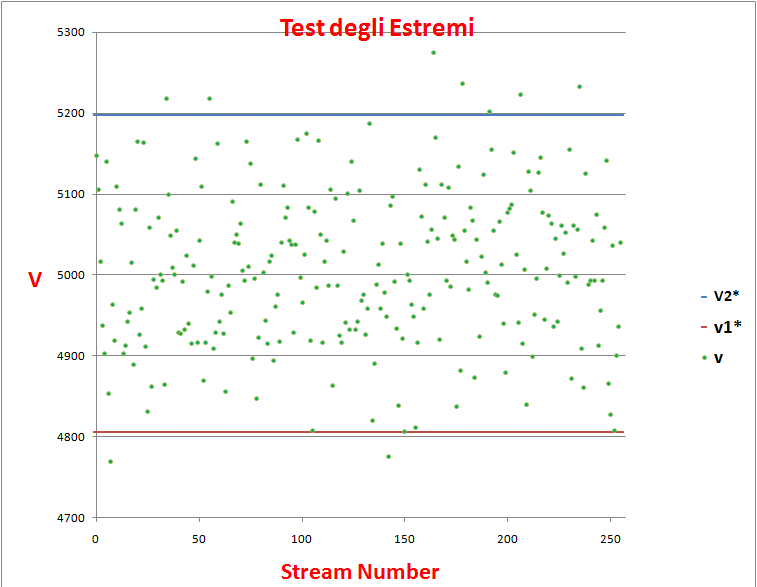
\includegraphics[scale=0.5]{img/result_37524306.png}
  \caption[Test degli estremi]{SEED 37524306.}
  \label{fig:result_37524306}
\end{figure}
\item 123456789
\begin{figure}[H]
  \centering
  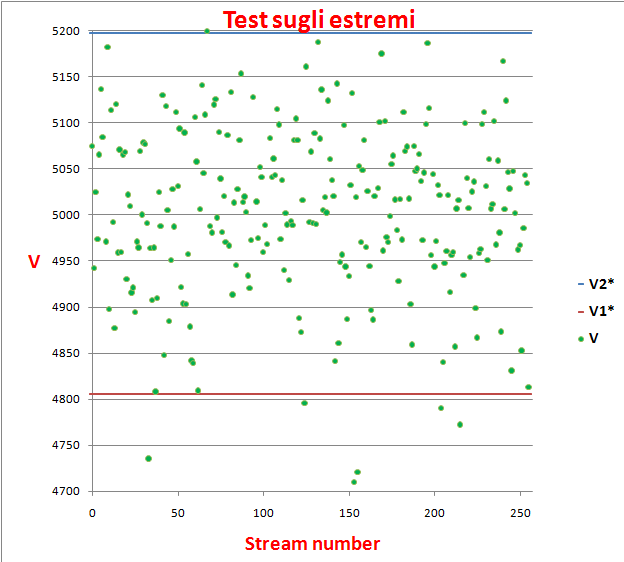
\includegraphics[scale=0.5]{img/result_123456789.png}
  \caption[Test degli estremi]{SEED 123456789.}
  \label{fig:result_123456789}
\end{figure}
\end{itemize}

\vspace{0.5cm}
Alla luce dei diagrammi rappresentati si può vedere che su 256 test effettuati (uno per ogni stream del generatore), la maggior parte non è fallita sottolineando la buona randomicità del generatore, in quanto le statistiche rappresentate sono contenute all'interno dell'intervallo rappresentato dal massimo e dal minimo valore critico ($v_{i}^{*}$).

